
\documentclass[aspectratio=169]{beamer}

% --- PAQUETES ---
\usepackage[utf8]{inputenc}
\usepackage[english]{babel}
\usepackage{graphicx}
\usepackage{booktabs}
\usepackage{multicol}
\usepackage{amsmath}
\usepackage{amssymb}
\usepackage{tikz}
\usepackage{pgf-pie}
\usetikzlibrary{positioning, arrows.meta, shapes, fit, calc}
\usepackage{pgfplots}
\pgfplotsset{compat=1.17}
\usepackage{hyperref}
\usepackage{url}

% --- TEMA Y ESTILO ---
\usetheme{Madrid}
\usecolortheme{default}

% Definición de colores
\definecolor{DeepBlue}{RGB}{0,51,102}
\definecolor{AlertRed}{RGB}{204,0,0}
\definecolor{SafeGreen}{RGB}{0,100,0}
\definecolor{OrangeAccent}{RGB}{230,126,34}

% --- METADATA ---
\title[Financial Networks]{Financial Networks \& Technological Innovation}

\author{Hernán Venegas}
\institute{Universidad de Los Andes}
\date{December 1, 2025}

\begin{document}

% -------------------------------------------------------------------
% SLIDE 1: PORTADA
% -------------------------------------------------------------------
\frame{\titlepage}

% ===================================================================
% SECCIÓN 1: MOTIVACIÓN
% ===================================================================
\section{Motivation}

\begin{frame}{Background: Economic Impact of non Traditional Networks}

\textbf{Market Size \& Projections:}

\begin{itemize}
    \item \alert{Shadow Banking (NBFI)}: \$238.8T in assets (2023)
    \begin{itemize}
        \item[-] Now \textbf{49.1\% of global financial system} (Financial Stability Board, 2024)
    \end{itemize}
    
    \vspace{0.3cm}
    
    \item \alert{Decentralized Finance (DeFi)}: Global Decentralized Finance Market size is expected to reach \$351.75 billion by 2031
    \begin{itemize}
        \item[-] Market growth of 48.9\% CAGR (Research and Markets, 2025)
    \end{itemize}
    
    \vspace{0.3cm}
    
    \item \alert{Fintech Lending}: Tripled US mortgage market share
    \begin{itemize}
        \item[-] 14\% (2007) → 38\% (2015) (Buchak et al., 2018)
    \end{itemize}
\end{itemize}

\vspace{0.4cm}

\begin{alertblock}{Research Gap}
\centering
Theory assumes \textit{single network} but reality shows \textit{dual coexistence}\\
\textbf{Our study: a dual-network equilibrium model}
\end{alertblock}

\end{frame}


\begin{frame}{Motivation: The Regulatory Constraint Problem}
    
    \textbf{The Problem:}
    \begin{itemize}
        \item Financial networks require connectivity for efficient risk pooling
        \item \textbf{Regulations} often prohibit specific direct links
        \item \textbf{Consequence:} 50.8\% welfare loss in our benchmark case
    \end{itemize}
    
    \vspace{0.5cm}
    \textbf{Questions:}
    \begin{itemize}
        \item Can the addition of a new central agent (high centrality) solve this?
        \item Can \textcolor{blue}{alternative infrastructure} do better?
        \item Will alternative networks replace or coexist with traditional systems?
        \item What determines adoption of these technologies?
    \end{itemize}

\end{frame}

\begin{frame}{Research Questions}
\textbf{Main questions we address:}
\begin{enumerate}
    \item Can a new central agent resolve structural inefficiencies from regulatory constraints?
    \item Can \textcolor{blue}{alternative infrastructure} achieve full welfare recovery?
    \item Under what conditions do agents \textcolor{blue}{adopt alternative networks}? When do we observe \textcolor{blue}{coexistence} vs. \textcolor{blue}{dominance}?
\end{enumerate}

\vspace{0.5cm}
\textbf{Our approach:} Extend Jalan et al. (2024) to model competing networks with different regulatory and technological characteristics.
\end{frame}

% ===================================================================
% SECCIÓN 2: MODELO BASE (JALAN ET AL.)
% ===================================================================
\section{Base Model}

\begin{frame}{Why This Base Model?}
\textbf{Objective:} Study endogenous formation of financial networks and impact of competing network emergence.

\vspace{0.5cm}
\textbf{Why Jalan et al. (2024)?}
\begin{itemize}
    \item Allows modeling \textcolor{blue}{endogenous network formation}
    \item Captures \textcolor{blue}{utility maximization} of heterogeneous agents
    \item Incorporates \textcolor{blue}{subjective beliefs} and differentiated risk aversion
    \item Provides \textcolor{blue}{existence and uniqueness conditions} for equilibrium
    \item Pairwise stability through bilateral negotiations
\end{itemize}

\vspace{0.3cm}
\textbf{Our contribution:} We extend the model to include a second network (alternative infrastructure) that competes with the traditional network in transparency and cost dimensions.
\end{frame}

\begin{frame}{Base Model: Network Structure}
\textbf{Network representation:} $n$ agents connected by weighted network $W\in\mathbb{R}^{n\times n}$

\vspace{0.3cm}
\textbf{Contract structure:}
\begin{itemize}
    \item \textbf{Contract sizes:} $W_{ij}$ = size of contract between agents $i$ and $j$
    \begin{itemize}
        \item Symmetric: $W_{ij} = W_{ji}$ (mutual agreement required)
        \item Can be positive, negative, or zero
    \end{itemize}
    
    \item \textbf{Contract pricing:} $P_{ji} = -P_{ij}$ (zero-sum payments)
    \begin{itemize}
        \item Payment amount: $P_{ji} \cdot W_{ji}$
        \item Allows side payments for agreement
    \end{itemize}
\end{itemize}

\vspace{0.3cm}
Contracts emerge endogenously from agent interactions, not imposed exogenously.
\vspace{0.2cm}
\textbf{Important:} The model doesn't consider capital raising.
\end{frame}

\begin{frame}{Agent Characteristics}
\textbf{Each agent $i$ is characterized by:}

\begin{itemize}
    \item \textbf{Subjective beliefs:} $\mu_i \in \mathbb{R}^n$
    \begin{itemize}
        \item Expected profitability from contracts with each agent
    \end{itemize}
    
    \item \textbf{Risk perception:} $\Sigma_i \succ 0$
    \begin{itemize}
        \item Covariance matrix of perceived risks
        \item Captures correlations between different contracts
    \end{itemize}
    
    \item \textbf{Risk preferences:} $\gamma_i > 0$
    \begin{itemize}
        \item Risk aversion parameter
    \end{itemize}
\end{itemize}

We define $J_i \subseteq [n]$ as the set of agents with whom agent $i$ can contract
\begin{itemize}
    \item \textbf{Constraints:} $\Psi_i \in \{0,1\}^{|J_i| \times n}$ where 
    \begin{itemize}
        \item Regulatory or operational limitations determines feasible contract set
    \end{itemize}
\end{itemize}
\end{frame}

\begin{frame}{Agent Behavior: Utility Maximization}
\textbf{Mean-variance utility function:}
\begin{equation}
g_i(W,P) = w_i^\top (\mu_i - P e_i) - \gamma_i \cdot w_i^\top \Sigma_i w_i
\end{equation}

\vspace{0.3cm}
\textbf{Economic interpretation:}
\begin{itemize}
    \item \textbf{Expected return:} $w_i^\top (\mu_i - P e_i)$
    \begin{itemize}
        \item $w_i$: agent $i$'s portfolio vector
        \item $\mu_i - P e_i$: net expected returns after prices
    \end{itemize}
    
    \item \textbf{Risk penalty:} $\gamma_i \cdot w_i^\top \Sigma_i w_i$
    \begin{itemize}
        \item Higher $\gamma_i$ → more risk-averse agent
        \item $\Sigma_i$: agent $i$'s perceived risk structure
    \end{itemize}
\end{itemize}

\vspace{0.3cm}
\textbf{Optimization:} Each agent chooses portfolio to maximize utility subject to constraints $\Psi_i$.
\end{frame}

\begin{frame}{Stable Network Formation}
\textbf{Optimal portfolio solution:}
$$w_i^* = Q_i(\mu_i - Pe_i)$$
where: $Q_i = \Psi_i^\top(2\gamma_i\Psi_i\Sigma_i\Psi_i^\top)^{-1}\Psi_i$

\vspace{0.3cm}
\textbf{Stability conditions:}
\begin{itemize}
    \item \textbf{Feasibility (definition 2):} $W = W^T$, $P = -P^T$, constraints satisfied
    \item \textbf{Stability (definition 3):} Each agent maximizes utility given a feasible (W, P)
\end{itemize}

\vspace{0.3cm}
\textbf{Convergence:} Iterative price updates until stable network emerges
\end{frame}

% ===================================================================
% SLIDES NUEVAS: ALGORITMO DE NEGOCIACIÓN
% ===================================================================

\begin{frame}{Network Formation: Bilateral Negotiations}
    \textbf{How does the network structure emerge?} \\
    It emerges from decentralized, iterative negotiations, capturing the nature of Over-the-Counter (OTC) markets.
    
    \begin{block}{Algorithm: Iterative Pairwise Negotiation}
        \textbf{Procedure} Pairwise($\eta \in (0,1)$):
        \begin{enumerate}
            \item Initialize $t \leftarrow 0$, $P(0) \leftarrow$ any skew-symmetric matrix
            \item \textbf{While} $P(t)$ has not converged \textbf{do}:
            \item \quad For all pairs $(i,j)$, compute negotiated price $P'_{ij}$
            \item \quad Update global prices (dampened update):
            $$P(t+1) \leftarrow (1 - \eta)P(t) + \eta P'$$
            \item \quad $t \leftarrow t+1$
            \item \textbf{End While}
        \end{enumerate}
    \end{block}
    
   
\end{frame}

\begin{frame}{The Original Mechanism}
    The negotiation of $P'_{ij}$ happens in two logical stages at each step:
    
    \vspace{0.3cm}
    \textbf{Stage 1: Portfolio Optimization (Internal)} \\
    Each agent $i$ calculates their optimal portfolio $w_i^*$ given current prices $P(t)$:
    \begin{equation}
        w_i^* = \Psi_i^\top (2\gamma_i \Psi_i \Sigma_i \Psi_i^\top)^{-1} \Psi_i (\mu_i - P e_i)
    \end{equation}
    \tiny{\textit{*Constraints $\Psi_i$ are applied here, forcing zero volume on prohibited links.}}
    
    \vspace{0.3cm}
    \normalsize
    \textbf{Stage 2: Price Discovery (Bilateral)} \\
    If agents disagree on contract size ($w_{ij}^* \neq w_{ji}^*$), the price adjusts to close the gap:
    \begin{equation}
        P_{ij}^{new} = P_{ij}^{old} + \eta \cdot \frac{Q_j[\mu_j - P e_j]_{ij} - Q_i[\mu_i - P e_i]_{ji}}{Q_{ii} + Q_{jj}}
    \end{equation}
    \vspace{0.1cm}
    \small{Prices change to compensate the agent who needs more incentive to accept the volume.}
\end{frame}


\begin{frame}{Principal Metrics that we use}

    \vspace{-0.5cm}
    \begin{columns}[T]
        \column{0.5\textwidth}
        \begin{block}{1. Bilateral Volume ($V$) }
            Measures total activity, no self-investment.
            $$V = \frac{1}{2} \left( \sum_{i=1}^N \sum_{j=1}^N |W_{ij}| - \sum_{i=1}^N |W_{ii}| \right)$$
        \end{block}
        
        \begin{block}{2. Welfare (Utility $U_i$ \& $U_{Total}$)}
            \textbf{Agent Utility ($U_i$):} Risk-adjusted benefit.
            $$U_i = w_i^\top (\mu_i - P e_i) - \gamma_i w_i^\top \Sigma_i w_i$$
            \textbf{Total Welfare:} The sum of all agents' utilities.
            $$U_{Total} = \sum_{i} U_i$$
        \end{block}
        
        \column{0.45\textwidth}
        \begin{block}{3. Net Rents ($R_i$)}
            Measures payments.
            $$R_i = \sum_{j} P_{ji} W_{ji}$$
            
            \textbf{Interpretation:}
            \begin{itemize}
                \item \textcolor{SafeGreen}{$R_i > 0$}: Net Reciever of payments (Extracts value)
                \item \textcolor{AlertRed}{$R_i < 0$}: Net Payer 
            \end{itemize}
        \end{block}
        
    \end{columns}
\end{frame}

\begin{frame}{Original Example 5 from Jalan et al (2024)}
    \small
    Three agents with potential gains from trade, where the direct link between the \textbf{National Bank (1)} and the \textbf{Local Firm (3)} is blocked.
    
    \begin{columns}[T]
        % --- COLUMNA IZQUIERDA: PARÁMETROS ECONÓMICOS ---
        \column{0.45\textwidth}
            \begin{block}{1. Parameters ($M, \Sigma$)}
                \textbf{Expected Returns ($M$):}
                $$
                M = \begin{bmatrix} 
                    0 & 0.9 & \textcolor{red}{\mathbf{0.9}} \\ 
                    0.75 & 0 & 0.95 \\ 
                    0.5 & 0.8 & 0 
                \end{bmatrix}
                $$
                \footnotesize{\textit{Observation: $M_{13}=0.9$ indicates the expected return for the Local Firm (agent 3) for a contract with the National Bank (agent 1), but this link is prohibited.}}
                
                \vspace{0.2cm}
                \textbf{Risk:} Symmetric covariance ($\Sigma_1=\Sigma_2=\Sigma_3$) and risk aversion $\gamma_i=1$ for all agents.
            \end{block}

        % --- COLUMNA DERECHA: RESTRICCIONES ESTRUCTURALES ---
        \column{0.52\textwidth}
            \begin{block}{2. Regulatory Constraints ($\Psi$)}
                The matrices $\Psi_i$ restrict the optimization set, forcing specific contract weights to zero ($w_{ij}=0$).
                
                \vspace{0.2cm}
                \textbf{Agent 1 (National Bank):} 
                Cannot contract with Agent 3.
                $$ \Psi_1 = \begin{bmatrix} 1 & 0 & 0 \\ 0 & 1 & 0 \end{bmatrix} $$
                
                \textbf{Agent 3 (Local Firm):} 
                Cannot contract with Agent 1.
                $$ \Psi_3 = \begin{bmatrix} 0 & 1 & 0 \\ 0 & 0 & 1 \end{bmatrix} $$
                
                \textbf{Agent 2 (Local Bank):} 
                Unconstrained ($\Psi_2 = I_3$).
            \end{block}
    \end{columns}
\end{frame}


\begin{frame}{Original Example 5 from Jalan et al (2024)}
    % --- PARTE SUPERIOR: Contexto (Ancho completo) ---
    
    \begin{itemize}
        \item \textbf{Constraint:} The direct link NB $\leftrightarrow$ LF is \textcolor{AlertRed}{prohibited}.
        \item \textbf{Outcome:} The Local Bank becomes a central bottleneck. Stable equilibrium is reached in $\sim$10 iterations.
    \end{itemize}
    

    % --- PARTE INFERIOR: Columnas (75% Imagen / 25% Matrices) ---
    \begin{columns}[T] % Alineación superior
        
        % COLUMNA IZQUIERDA (75%): Diagrama de Topología GRANDE
        \column{0.7\textwidth}
            \centering
            
            \textbf{\scriptsize Equilibrium Contracts ($W$)}
            
\includegraphics[width=\linewidth, keepaspectratio]{docs/Diapos/W_original.png}
            
            \vspace{0.2cm}
            
            \textbf{\scriptsize Equilibrium Prices ($P$)}
            
\includegraphics[width=\linewidth, keepaspectratio]{docs/Diapos/P_original.png}
            

        % COLUMNA DERECHA (25%): Matrices pequeñas
        \column{0.25\textwidth}
            \centering
            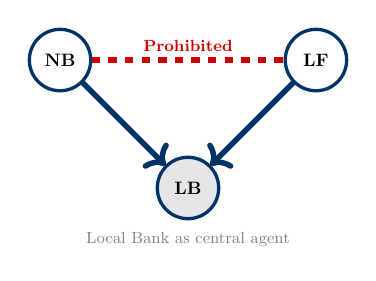
\begin{tikzpicture}[scale=0.65, transform shape] % Escala aumentada
                % Nodos
                \node[circle, draw=DeepBlue, very thick, minimum size=1.2cm, fill=white] (NB) at (0,3) {\textbf{NB}};
                \node[circle, draw=DeepBlue, very thick, minimum size=1.2cm, fill=white] (LF) at (5,3) {\textbf{LF}};
                \node[circle, draw=DeepBlue, very thick, minimum size=1.2cm, fill=gray!20] (LB) at (2.5,0.5) {\textbf{LB}};
                
                % Conexiones
                \draw[AlertRed, line width=2.5pt, dashed] (NB) -- (LF) node[midway, above, font=\small, text=AlertRed] {\textbf{Prohibited}};
                \draw[->, line width=2pt, DeepBlue] (NB) -- (LB);
                \draw[->, line width=2pt, DeepBlue] (LF) -- (LB);
                
                % Etiquetas
                \node[font=\small, text=gray] at (2.5, -0.5) {Local Bank as central agent};
            \end{tikzpicture}
            The Local Bank gets a contract $W=0.26$ with the National Bank and $W=0.56$ with the Local Firm. With $P=-0.26$ and $P=-0.23$, respectively.
    \end{columns}
\end{frame}

\begin{frame}{Extension of the Example 5: Unrestricted Scenario}
    % --- PARTE SUPERIOR: Contexto (Ancho completo) ---
    
    Now we only take out the restrictions ($\Psi_1=\Psi_2=\Psi_3=I_3$). This will be our benchmark $w^*$ from now on, the scenario without restrictions.
    

    % --- PARTE INFERIOR: Columnas (75% Imagen / 25% Matrices) ---
    \begin{columns}[T] % Alineación superior
        
        % COLUMNA IZQUIERDA (75%): Diagrama de Topología GRANDE
        \column{0.7\textwidth}
            \centering
            
            \textbf{\scriptsize Equilibrium Contracts ($W$)}
            
\includegraphics[width=\linewidth, keepaspectratio]{docs/Diapos/W_original_SR.png}
            
            \vspace{0.2cm}
            
            \textbf{\scriptsize Equilibrium Prices ($P$)}
            
\includegraphics[width=\linewidth, keepaspectratio]{docs/Diapos/P_original_SR.png}
            

        % COLUMNA DERECHA (25%): Matrices pequeñas
        \column{0.25\textwidth}
            \centering
            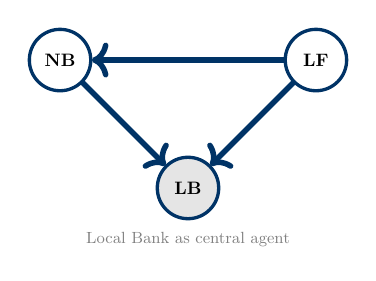
\begin{tikzpicture}[scale=0.65, transform shape] % Escala aumentada
                % Nodos
                \node[circle, draw=DeepBlue, very thick, minimum size=1.2cm, fill=white] (NB) at (0,3) {\textbf{NB}};
                \node[circle, draw=DeepBlue, very thick, minimum size=1.2cm, fill=white] (LF) at (5,3) {\textbf{LF}};
                \node[circle, draw=DeepBlue, very thick, minimum size=1.2cm, fill=gray!20] (LB) at (2.5,0.5) {\textbf{LB}};
                
                % Conexiones
                \draw[->, line width=2pt, DeepBlue] (NB) -- (LB);
                \draw[->, line width=2pt, DeepBlue] (LF) -- (LB);
                \draw[->, line width=2pt, DeepBlue] (LF) -- (NB);
                
                % Etiquetas
                \node[font=\small, text=gray] at (2.5, -0.5) {Local Bank as central agent};
            \end{tikzpicture}
            Now the Local Bank gets a contract $W=-0.07$ with the National Bank and $W=0.88$ with the Local Firm. With $P=-0.03$ and $P=-0.24$, respectively.
    \end{columns}
\end{frame}

% ===================================================================
% SECCIÓN 3: EL PROBLEMA
% ===================================================================
\section{The Problem}


\begin{frame}{Impact of the Constraint}
    We compare the scenarios with and without the restriction between the National Bank and the Local Firm.
    
    \vspace{0.3cm}
    \begin{columns}
        \column{0.5\textwidth}
        \textbf{Impact of Constraint:}
        \begin{itemize}
            \item \textbf{Bilateral Volume:} 0.822 (vs 1.976 unconstrained)
            \item \textbf{Activity Loss:} \textcolor{red}{\textbf{58.4\%}}
            \item \textbf{Total Welfare:} 0.706 (vs 1.434 unconstrained)
            \item \textbf{Welfare Loss:} \textcolor{red}{\textbf{50.8\%}}
        \end{itemize}
        
        \vspace{0.3cm}
        \textbf{Who suffers most?}
        \begin{itemize}
            \item Local Firm: -66.1\% utility
            \item National Bank: -84.6\% utility
            \item Local Bank: \textcolor{SafeGreen}{+3.6\%} 
        \end{itemize}
        
        \column{0.5\textwidth}
        \centering
        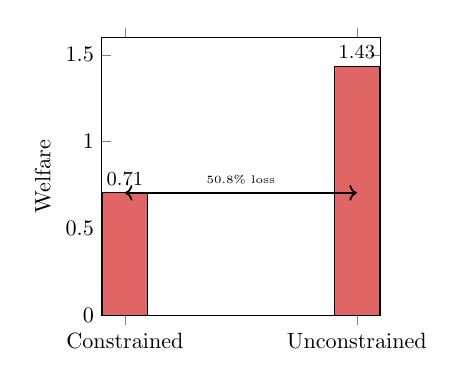
\begin{tikzpicture}[scale=0.8]
            \begin{axis}[
                ybar,
                bar width=20pt,
                ylabel={Welfare},
                symbolic x coords={Constrained, Unconstrained},
                xtick=data,
                ymin=0, ymax=1.6,
                height=6cm, width=6cm,
                nodes near coords,
                every node near coord/.append style={font=\small},
                legend style={at={(0.5,-0.2)}, anchor=north}
            ]
            \addplot[fill=AlertRed!60] coordinates {(Constrained,0.706) (Unconstrained,1.434)};
            \draw[<->, thick] (axis cs:Constrained,0.706) -- (axis cs:Unconstrained,0.706) node[midway, above, font=\tiny] {50.8\% loss};
            \end{axis}
        \end{tikzpicture}
        
        \vspace{0.3cm}
        \small{\textit{Half of potential welfare is erased by the constraint}}
    \end{columns}
\end{frame}

% ===================================================================
% SECCIÓN 4: SOLUCIÓN 1 - COMPETENCIA
% ===================================================================


\section{Solution 1: Competition}

\begin{frame}{Extension: Adding Competition (Fintech Entry)}
    \textbf{Hypothesis:} Can adding a competitor reduce the inefficiency without removing the constraint?
    
    \begin{columns}[T]
        % --- COLUMNA IZQUIERDA: LÓGICA DEL EXPERIMENTO ---
        \column{0.55\textwidth}
            \begin{block}{The "Clone" Competitor}
                We introduce \textbf{Firm 4 (Fintech)} to compete with the Local Bank. To isolate the pure effect of competition, we design it as a near-perfect substitute.
                
                \begin{itemize}
                    \item Agent with access to every other agent.
                    \item \textbf{Constraint:} Direct link NB $\leftrightarrow$ LF remains \textcolor{AlertRed}{blocked}.
                    \item \textbf{Symmetry:} Same risk profile and expected returns as the Local Bank.
                \end{itemize}
            \end{block}
            
        % --- COLUMNA DERECHA: MATEMÁTICAS Y VISUALIZACIÓN ---
        \column{0.48\textwidth}
            \centering
            
            % DIAGRAMA TIKZ (TOPOLOGÍA DIAMANTE)
            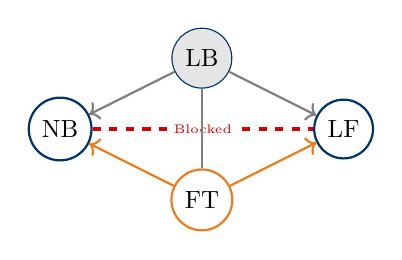
\begin{tikzpicture}[scale=0.9, transform shape]
                % Nodos
                \node[circle, draw=DeepBlue, thick, fill=white] (NB) at (0,2) {NB};
                \node[circle, draw=DeepBlue, thick, fill=white] (LF) at (4,2) {LF};
                
                \node[circle, draw=DeepBlue, fill=gray!20] (LB) at (2,3) {LB};
                \node[circle, draw=OrangeAccent, thick, fill=white] (FT) at (2,1) {FT};
                
                % Conexiones
                \draw[AlertRed, line width=1.5pt, dashed] (NB) -- (LF) node[midway, fill=white, inner sep=1pt, font=\tiny, text=AlertRed] {Blocked};
                
                \draw[->, thick, gray] (LB) -- (NB);
                \draw[->, thick, gray] (LB) -- (LF);
                \draw[-, thick, gray] (LB) -- (FT);
                \draw[->, thick, OrangeAccent] (FT) -- (NB);
                \draw[->, thick, OrangeAccent] (FT) -- (LF);
                
            \end{tikzpicture}
            
            
            % MATRIZ DE COVARIANZA
            \textbf{\footnotesize New Covariance Matrix ($\Sigma$)}
            $$
            \Sigma = \begin{bmatrix} 
                1.0 & 0.25 & 0.75 & 0.25 \\ 
                0.25 & \mathbf{1.0} & 0.60 & \textcolor{OrangeAccent}{\mathbf{0.99}} \\ 
                0.75 & 0.60 & 1.0 & 0.60 \\ 
                0.25 & \textcolor{OrangeAccent}{\mathbf{0.99}} & 0.60 & \mathbf{1.0} 
            \end{bmatrix}
            $$

            
    \end{columns}
    High correlation ($\rho = 0.99$) between Fintech and Local Bank ensures they are seen as "the same" by the network. It isn't $\rho =1$ beacuase we would have a singular matrix.
\end{frame}

\begin{frame}{Solution 1: Add Competition (Fintech Entry)}
    \textbf{Logic:} Competition should reduce monopolistic rents and improve efficiency
    
    \vspace{0.3cm}
    \begin{table}
        \centering
        \small
        \begin{tabular}{lcccc}
            \toprule
            \textbf{Metric} & \textbf{3F-WITH} & \textbf{4F-WITH} & \textbf{Gain} & \textbf{vs Ideal} \\
            \midrule
            Bilateral Volume & 0.822 & 1.351 & +64.3\% & \textcolor{red}{-31.6\%} \\
            Total Welfare & 0.706 & 1.034 & +46.5\% & \textcolor{red}{-27.9\%} \\
            \midrule
            \textit{Agent Utilities} \\
            Local Firm & 0.202 & 0.391 & +93.6\% & \textcolor{red}{-54.7\%} \\
            Local Bank & 0.441 & 0.239 & -45.7\% & \textcolor{red}{-27.1\%} \\
            Fintech & --- & 0.239 & --- & --- \\
            National Bank & 0.064 & 0.165 & +159.6\% & \textcolor{red}{-31.8\%} \\
            \bottomrule
        \end{tabular}
    \end{table}
    
    \vspace{0.3cm}
    \begin{alertblock}{Key Finding}
        Competition helps but \textbf{cannot overcome structural constraint}. \\
        Persistent welfare gap: \textcolor{red}{\textbf{27.9\%}} vs 3-agent ideal
    \end{alertblock}
\end{frame}
\begin{frame}{Solution 1: Add Competition (Fintech Entry)}
    The key change when adding a new agent is in the payments flows. 
    
    \begin{table}[h]
\centering
\caption{Impact of Fintech Entry on Network Activity and Welfare}
\label{tab:fintech_impact}
\begin{tabular}{lcc}
\hline
\textit{\textbf{Rent Decomposition (Net Payments)}} & &  \\
Rents (National Bank) & 0.0681 & -0.0146  \\
Rents (Local Bank) & -0.1977 & 0.0256  \\
Rents (Local Firm) & 0.1297 & -0.0365  \\
Rents (Fintech) & -- & 0.0256  \\ \hline
\textbf{Total System Rents} & \textbf{0.000} & \textbf{0.000} \\
\hline
\end{tabular}
\end{table}
Why the payments flows change?

\end{frame}


\begin{frame}{Why Competition Fails: The Structural Bottleneck}
    \begin{columns}
        \column{0.5\textwidth}
        \textbf{What competition achieves:}
        \begin{itemize}
            \item \textcolor{SafeGreen}{Increase activity and total welfare}
            \item \textcolor{SafeGreen}{Lowers prices}
            \item \textcolor{SafeGreen}{Improves Local Firm and National Bank utilities}
        \end{itemize}
        
        \vspace{0.3cm}
        \textbf{What competition cannot fix:}
        \begin{itemize}
            \item \textcolor{red}{Biggest contract remains blocked}
            \item \textcolor{red}{Forced central agents persists}
            \item \textcolor{red}{Structural inefficiency remains}
        \end{itemize}
        
        \vspace{0.3cm}
        Competition is \textbf{good but insufficient}
        
        \column{0.5\textwidth}
        \centering
        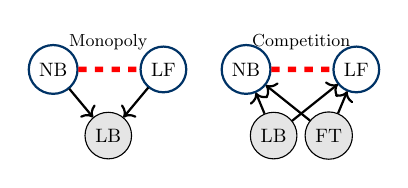
\begin{tikzpicture}[scale=0.7, transform shape]
            % Monopoly
            \node[font=\small] at (0, 3.5) {Monopoly};
            \node[circle, draw=DeepBlue, thick, minimum size=0.6cm] (NB1) at (-1,3) {NB};
            \node[circle, draw=DeepBlue, thick, minimum size=0.6cm] (LF1) at (1,3) {LF};
            \draw[red, line width=2pt, dashed] (NB1) -- (LF1);
            \node[circle, draw, fill=gray!20, minimum size=0.6cm] (B1) at (0,1.8) {LB};
            \draw[->, thick] (NB1) -- (B1);
            \draw[->, thick] (LF1) -- (B1);
            
            % Competition
            \node[font=\small] at (3.5, 3.5) {Competition};
            \node[circle, draw=DeepBlue, thick, minimum size=0.6cm] (NB2) at (2.5,3) {NB};
            \node[circle, draw=DeepBlue, thick, minimum size=0.6cm] (LF2) at (4.5,3) {LF};
            \draw[red, line width=2pt, dashed] (NB2) -- (LF2);
            \node[circle, draw, fill=gray!20, minimum size=0.5cm] (B2) at (3,1.8) {LB};
            \node[circle, draw, fill=gray!20, minimum size=0.5cm] (F2) at (4,1.8) {FT};
            \draw[->, thick] (B2) -- (NB2);
            \draw[->, thick] (B2) -- (LF2);
            \draw[->, thick] (F2) -- (NB2);
            \draw[->, thick] (F2) -- (LF2);
        \end{tikzpicture}
        
        \vspace{0.3cm}
        \small{\textit{Competition divides utilities but \\
        cannot remove structural bottleneck}}
    \end{columns}
\end{frame}

\begin{frame}{The Natural Response: Alternative Infrastructure Emerges}
    \textbf{Historical pattern:} When regulations create inefficiencies, markets develop workarounds
    
    \vspace{0.3cm}
    \begin{columns}
        \column{0.5\textwidth}
        \textbf{Documented examples:}
        \begin{itemize}
            \item \textbf{Shadow Banking:}
            \begin{itemize}
                \item Market share doubled 2007-2015
                \item Operates outside regulated perimeter
                \item Legally distinct from "banks"
            \end{itemize}
            
            \item \textbf{Offshore Financial Centers:}
            \begin{itemize}
                \item Jurisdiction arbitrage
                \item Alternative regulatory frameworks
            \end{itemize}
            
            \item \textbf{Fintech Platforms:}
            \begin{itemize}
                \item P2P lending, DeFi protocols
                \item Operate in different legal categories
            \end{itemize}
        \end{itemize}
        
        
        \column{0.5\textwidth}
        
        \vspace{0.3cm}
        \centering
        \textbf{Shadow Banking Growth Decomposition}
        
        \vspace{0.2cm}
        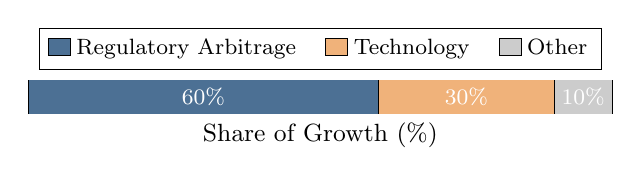
\begin{tikzpicture}
        \begin{axis}[
            xbar stacked,
            width=9cm,
            height=2cm,
            xmin=0, xmax=100,
            xlabel={\small Share of Growth (\%)},
            xlabel style={font=\small},
            ytick=\empty,
            xtick=\empty,
            enlarge y limits=0.5,
            bar width=1cm,
            nodes near coords={\pgfmathprintnumber\pgfplotspointmeta\%},
            nodes near coords align={center},
            every node near coord/.append style={font=\footnotesize, text=white},
            legend style={
                at={(0.5,1.3)},          % ARRIBA: y > 1
                anchor=south,
                legend columns=3,
                font=\footnotesize,
                /tikz/every even column/.append style={column sep=0.3cm}
            },
        ]
        \addplot[fill=DeepBlue!70, draw=black, line width=0.3pt] coordinates {(60,0)};
        \addplot[fill=OrangeAccent!60, draw=black, line width=0.3pt] coordinates {(30,0)};
        \addplot[fill=gray!40, draw=black, line width=0.3pt] coordinates {(10,0)};
        \legend{Regulatory Arbitrage, Technology, Other}
        \end{axis}
    \end{tikzpicture}
        
        \vspace{0.3cm}
        \begin{block}{Buchak et al. (2018) shadow banking:}
            \small
            60\% of shadow bank growth from regulatory differences, 30\% from technology
            
            \vspace{0.2cm}
            \textit{Regulatory constraints are the primary driver of alternative network adoption}
        \end{block}
    \end{columns}
\end{frame}


\begin{frame}{From Empirics to Theory: Modeling the Phenomenon}
    \textbf{Given that alternative networks emerge empirically, what are the welfare implications?}
    
    \vspace{0.3cm}
    \begin{columns}
        \column{0.55\textwidth}
        \textbf{What we know:}
        \begin{enumerate}
            \item Regulations create structural inefficiencies
            
            \item Competition helps but is insufficient (gap persists)
            
            \item Alternative infrastructure emerges in practice (shadow banking, fintech, offshore)
            
            \item Regulatory arbitrage dominates technology as adoption driver (60\% vs 30\%)
        \end{enumerate}
        
        \vspace{0.3cm}
        \textbf{What we ask:}
        \begin{itemize}
            \item Can these alternatives restore lost welfare?
            \item Under what conditions?
            \item What determines adoption patterns?
        \end{itemize}
        
        \column{0.45\textwidth}
        \centering
        \textbf{Our contribution:}
        
        \vspace{0.3cm}
        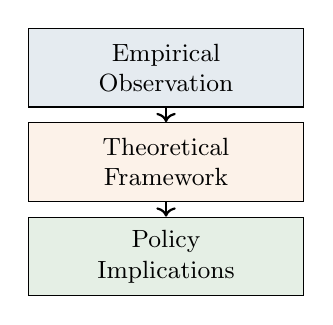
\begin{tikzpicture}[scale=0.8, every node/.style={font=\small}]
            % Boxes
            \node[draw, rectangle, fill=DeepBlue!10, align=center, minimum width=3.5cm, minimum height=1cm] (empirics) at (0,3) {Empirical\\Observation};
            
            \node[draw, rectangle, fill=OrangeAccent!10, align=center, minimum width=3.5cm, minimum height=1cm] (theory) at (0,1.5) {Theoretical\\Framework};
            
            \node[draw, rectangle, fill=SafeGreen!10, align=center, minimum width=3.5cm, minimum height=1cm] (policy) at (0,0) {Policy\\Implications};
            
            % Arrows
            \draw[->, thick] (empirics) -- (theory);
            \draw[->, thick] (theory) -- (policy);
        \end{tikzpicture}
        
        \vspace{0.3cm}
        \small{We formalize this empirical phenomenon to derive optimal policy responses}
    \end{columns}
\end{frame}

\begin{frame}{Why Competition Alone Is Insufficient}
    \textbf{Before modeling alternative networks, why can't competition solve the problem?}
    
    \vspace{0.3cm}
    \begin{columns}
        \column{0.45\textwidth}
        \textbf{What competition achieves:}
        \begin{itemize}
            \item \textcolor{SafeGreen}{Reduces monopoly rents}
            \item \textcolor{SafeGreen}{Lowers intermediation costs}
            \item \textcolor{SafeGreen}{Improves welfare (+46.5\%)}
        \end{itemize}
        
        \vspace{0.3cm}
        \textbf{Fundamental limitation:}
        \begin{itemize}
            \item \textcolor{red}{Constraint remains}
            \item \textcolor{red}{27.9\% welfare gap still exists}
        \end{itemize}
        
            
        \column{0.55\textwidth}
        \centering
        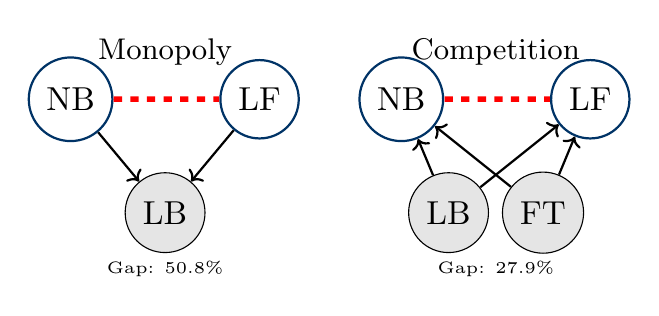
\begin{tikzpicture}[scale=1.2, transform shape]
            % Monopoly
            \node[font=\small] at (0, 3.5) {Monopoly};
            \node[circle, draw=DeepBlue, thick, minimum size=0.6cm] (NB1) at (-1,3) {NB};
            \node[circle, draw=DeepBlue, thick, minimum size=0.6cm] (LF1) at (1,3) {LF};
            \draw[red, line width=2pt, dashed] (NB1) -- (LF1);
            \node[circle, draw, fill=gray!20, minimum size=0.6cm] (B1) at (0,1.8) {LB};
            \draw[->, thick] (NB1) -- (B1);
            \draw[->, thick] (LF1) -- (B1);
            \node[font=\tiny] at (0, 1.2) {Gap: 50.8\%};
            
            % Competition
            \node[font=\small] at (3.5, 3.5) {Competition};
            \node[circle, draw=DeepBlue, thick, minimum size=0.6cm] (NB2) at (2.5,3) {NB};
            \node[circle, draw=DeepBlue, thick, minimum size=0.6cm] (LF2) at (4.5,3) {LF};
            \draw[red, line width=2pt, dashed] (NB2) -- (LF2);
            \node[circle, draw, fill=gray!20, minimum size=0.5cm] (B2) at (3,1.8) {LB};
            \node[circle, draw, fill=gray!20, minimum size=0.5cm] (F2) at (4,1.8) {FT};
            \draw[->, thick] (B2) -- (NB2);
            \draw[->, thick] (B2) -- (LF2);
            \draw[->, thick] (F2) -- (NB2);
            \draw[->, thick] (F2) -- (LF2);
            \node[font=\tiny] at (3.5, 1.2) {Gap: 27.9\%};
        \end{tikzpicture}
        
        \vspace{0.3cm}
        \small{\textit{Structural bottleneck remains}}
    \end{columns}
\end{frame}

% ===================================================================
% SECTION: THE DUAL-NETWORK FRAMEWORK
% ===================================================================
\section{The Dual-Network Framework}

\begin{frame}{Model Extension: Dual Network Structure}
Now we extend the original model and add a second network, where agents can reallocate

\vspace{0.3cm}
\textbf{Network setting:} $(\mu_i, \gamma_i, \Sigma_i, \Psi_i^T, \Psi_i^A, \tau, \lambda_A)_{i \in [n]}$

\vspace{0.3cm}
\textbf{New parameters:}
\begin{itemize}
   \item $\Psi_i^T \in \{0,1\}^{|J_i^T| \times n}$: constraints in Traditional Network
   \item $\Psi_i^A \in \{0,1\}^{|J_i^A| \times n}$: constraints in Alternative Network
\end{itemize}
The other parameters are the same as in the original model
\begin{columns}[T]
        \column{0.5\textwidth}
        \begin{block}{1. Constraints ($\Psi$)}
            \begin{itemize}
                \item If $\Psi_i^T \neq \Psi_i^A \implies$ \textcolor{OrangeAccent}{\textbf{Regulatory Arbitrage}}.
            \end{itemize}
        \end{block}
        
        \column{0.45\textwidth}
        \begin{block}{2. Tech Parameters ($\tau, \lambda$)}
            \begin{itemize}
                \item $\tau \geq 0$: \textcolor{SafeGreen}{\textbf{Benefits}} (Transparency/Trust). Additive to returns.
                \item $\lambda_A \geq 0$: \textcolor{AlertRed}{\textbf{Frictions}} (Fees/Congestion). Quadratic cost.
            \end{itemize}
        \end{block}
    \end{columns}
    
    \vspace{0.2cm}
    \centering
    \footnotesize{The trade-off $\tau / \lambda_A$ determines the economic attractiveness of adoption.}
\end{frame}

% --- SLIDE 2: CORE INNOVATION ---
\begin{frame}{The Portfolio Constraint Approach}
    We model technological competition as a \textcolor{blue}{portfolio reallocation problem}, not a scaling problem.
    
    \vspace{0.3cm}
    
    We introduce an exogenous total portfolio $w_i^*$ (derived from the unconstrained case) that can be reallocated between the traditional and alternative network:
    
    \begin{equation}
        \boxed{w_i^* = w_i^T + w_i^A}
    \end{equation}
    
    \vspace{0.3cm}
    \begin{columns}[T]
        \column{0.48\textwidth}
        \textbf{Advantages:}
        \begin{enumerate}
            \item \textbf{Comparability:} Fixes total exposure, isolating technology effects.
            \item \textbf{Realism:} Reflects capital constraints (reallocation vs. expansion).
        \end{enumerate}
        
        \column{0.48\textwidth}
        \textbf{\phantom{Advantages:}}
        \begin{enumerate}
            \setcounter{enumi}{2}
            \item \textbf{Tractability:} Reduces to a single-variable optimization.
            \item \textbf{Intuition:} Captures the compositional nature of adoption.
        \end{enumerate}
    \end{columns}
\end{frame}

% --- SLIDE 4: UTILITY FUNCTION ---
\begin{frame}{Dual-Network Utility Function}
    Agent $i$'s total utility is the sum of utilities from both networks, subject to $w_i^T + w_i^A = w_i^*$.
    
    \begin{equation}
        g_i(w_i^T, w_i^A, P) = g_i^T(w_i^T, P) + g_i^A(w_i^A, P)
    \end{equation}
    
    \vspace{0.3cm}
    
    \textbf{Traditional Utility} 
    $$g_i^T = (w_i^T)^\top(\mu_i - Pe_i) - \gamma_i(w_i^T)^\top\Sigma_i w_i^T$$
    
    \vspace{0.2cm}
    
    \textbf{Alternative Utility}
    $$g_i^A = (w_i^A)^\top(\mu_i + \textcolor{SafeGreen}{\mathbf{\tau \mathbf{1}}} - Pe_i) - \gamma_i(w_i^A)^\top\Sigma_i w_i^A - \textcolor{AlertRed}{\mathbf{\lambda_A\|w_i^A\|^2}}$$
    
    \vspace{0.2cm}
    \small{\textit{The quadratic friction $\lambda_A\|w_i^A\|^2$ penalizes large volumes}}
\end{frame}

% --- SLIDE 5: EQUILIBRIUM DEFINITIONS ---
\begin{frame}{Equilibrium Definitions}
    \textbf{Definition: Dual-Network Feasible Point} \\
    A tuple $(W^T, W^A, P)$ satisfying:
    \begin{enumerate}
        \item Symmetry \& Price Consistency ($P$ applies to both).
        \item Compliance: $W^T$ respects $\Psi^T$, $W^A$ respects $\Psi^A$.
        \item \textbf{Constraint:} $w_i^T + w_i^A = w_i^*$ for all $i$.
    \end{enumerate}
    
    \vspace{0.4cm}
    
    \textbf{Definition: Dual-Network Stable Point} \\
    A feasible point where each agent maximizes utility by choosing $w_i^T$ optimally, with $w_i^A$ determined residually.
    
    \begin{equation}
        g_i(W^T, P) = \max_{w_i^T} \ g_i(w_i^T, w_i^* - w_i^T, P)
    \end{equation}
\end{frame}

% --- SLIDE 6: OPTIMAL ALLOCATION (THE RESULT) ---
\begin{frame}{Proposition: Optimal Allocation}
    Solving this yields the solution for the Traditional Network allocation:
    
    \begin{equation}
        \boxed{w_i^{T*} = Q_i^{\text{dual}} \cdot a_i}
    \end{equation}
    
    \vspace{0.3cm}
    
    \begin{columns}[T]
        \column{0.5\textwidth}
        \textbf{The Dual Q-Matrix:}
        $$Q_i^{\text{dual}} = (2\gamma_i\Sigma_i + \textcolor{AlertRed}{\mathbf{\lambda_A I}})^{-1}$$
        \footnotesize{(Simplified assuming $\Psi^T = I_n$)}
        
        \column{0.5\textwidth}
        \textbf{The Offset Vector:}
        $$a_i = -\tau \mathbf{1} + 2\gamma_i\Sigma_i w_i^* + 2\lambda_A w_i^*$$
        \footnotesize{Captures net effect of benefits and constraints.}
    \end{columns}
\end{frame}

% --- SLIDE 7: ECONOMIC INTERPRETATION ---
\begin{frame}{Our Extension: The Dual Q-Matrix}
    Comparing the structural matrices reveals the impact of the alternative network technology:
    
    \begin{align*}
        Q_i^{\text{original}} &= (2\gamma_i\Sigma_i)^{-1} \\
        Q_i^{\text{dual}} &= (2\gamma_i\Sigma_i + \textcolor{AlertRed}{\mathbf{\lambda_A I}})^{-1}
    \end{align*}
    
    \vspace{0.3cm}
    
    \begin{block}{Implications of $\lambda_A$}
        \begin{enumerate}
            \item \textbf{Implicit Risk Aversion:} The friction $\lambda_A$ is mathematically equivalent to an increase in risk aversion.
            \item \textbf{Reduced Responsiveness:} Agents become less sensitive to profit opportunities in the traditional network due to the "shadow cost" of the alternative option.
            \item \textbf{Spillovers:} Tech parameters ($\tau, \lambda_A$) alter traditional portfolios ($w^T$) even for non-adopters.
        \end{enumerate}
    \end{block}
\end{frame}
% ===================================================================
% SECCIÓN 5: EXTENSIÓN A DOS REDES
% ===================================================================



\begin{frame}{Replication: Symmetric Case (No Constraints)}
  
\includegraphics[width=\textwidth,height=0.65\textheight,keepaspectratio]{docs/Diapos/W_dual_SR.png}
  
  \begin{columns}[T]
    \begin{column}{0.55\textwidth}
      \textbf{No Restrictions Case}
      \begin{itemize}
        \item $\Psi_i^T = \Psi_i^A = I_3$
        \item No transparency and no friction $\tau = 0, \lambda_A = 0$
      \end{itemize}
      
      \vspace{0.2cm}
      \textbf{Prediction:} 50/50 split (
    \end{column}
    \begin{column}{0.45\textwidth}
      \begin{table}[h]
        \centering
        \begin{tabular}{|l|c|}
          \hline
          Traditional Volume  & 0.990 \\
          \hline
          Alternative Volume   & 0.990 \\
          \hline
          Total Bilateral Volume       & 1.980 \\
          \hline
          Alternative Adoption & 50.0\% \\
          \hline
          Total Welfare & 1.434 \\
          \hline
        \end{tabular}
      \end{table}
    \end{column}
  \end{columns}
  
  \small{\textit{Framework validated: symmetric networks produce symmetric allocation}}
\end{frame}

% ===================================================================
% SECCIÓN 6: SOLUCIÓN 2 - RED ALTERNATIVA
% ===================================================================
\section{Solution 2: Alternative Network}

\begin{frame}{Original Example 5 in Two Networks}
  
\includegraphics[width=\textwidth,height=0.65\textheight,keepaspectratio]{docs/Diapos/W_dual_CR.png}
  
  \begin{columns}[T]
    \begin{column}{0.55\textwidth}
      \textbf{Restricted Case}
      \begin{itemize}
        \item National Bank-Local Firm link is prohibited in Traditional
        \item No transparency and no friction $\tau = 0, \lambda_A = 0$
      \end{itemize}
      
      \textbf{Result:} Migration to Alternative Network
    \end{column}
    \begin{column}{0.45\textwidth}
      \begin{table}[h]
        \centering
        \begin{tabular}{|l|c|}
          \hline
          Traditional Volume  & 0.568 \\
          \hline
          Alternative Volume   & 1.486 \\
          \hline
          Total Bilateral Volume       & 2.054 \\
          \hline
          Alternative Adoption & 72.4\% \\
          \hline
          Total Welfare & 1.434 \\
          \hline
        \end{tabular}
      \end{table}
    \end{column}
  \end{columns}
  
  \vspace{0.3cm}
  \small{\textit{Blocked link migrates to Alternative Network, achieving full welfare recovery}}
\end{frame}

\begin{frame}{Result 1: Complete Welfare Recovery}
    \textbf{Finding:} Alternative Network achieves \textbf{100\% welfare recovery}
    
    \vspace{0.3cm}
    \begin{table}
        \centering
        \begin{tabular}{lccc}
            \toprule
            \textbf{Scenario} & \textbf{Welfare} & \textbf{vs Ideal} \\
            \midrule
            (3F-WITH) & 0.706 & -50.8\%  \\
            (4F-WITH) & 1.034 & -27.9\%  \\
            \midrule
            \textbf{3-Dual Network} & \textbf{1.434} & \textbf{0.0\%}  \\
            \midrule
            Ideal (3F-WITHOUT) & 1.434 & ---  \\
            \bottomrule
        \end{tabular}
    \end{table}
    
    \textbf{Coexistence}, not displacement: \\
    • Alternative Network: 72.4\% of bilateral volume (absorbs blocked link) \\
    • Traditional Network: 27.6\% of volume \\
    • Both networks operate simultaneously in equilibrium
\end{frame}

\begin{frame}{Result 2: Network Allocation Patterns}
    \textbf{How do agents allocate across networks?}
    
    \vspace{0.3cm}
    \begin{columns}
        \column{0.5\textwidth}
        \textbf{3-Agent Case (Monopoly):}
        \begin{itemize}
            \item Alternative adoption: \textcolor{blue}{\textbf{72.4\%}}
            \item Traditional volume: 0.568
            \item Alternative volume: 1.486
        \end{itemize}
        
        \vspace{0.3cm}
        \textbf{4-Agent Case (Competition):}
        \begin{itemize}
            \item Alternative adoption: \textcolor{blue}{\textbf{47.9\%}}
            \item Traditional volume: 1.567 (+176\%)
            \item Alternative volume: 1.442
            \item Lower migration: competition improves Traditional
        \end{itemize}
        
        \column{0.5\textwidth}
        \centering
        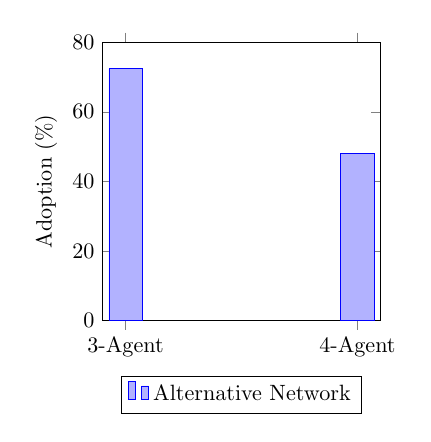
\begin{tikzpicture}[scale=0.8]
            \begin{axis}[
                ybar,
                bar width=15pt,
                ylabel={Adoption (\%)},
                symbolic x coords={3-Agent, 4-Agent},
                xtick=data,
                ymin=0, ymax=80,
                height=6cm, width=6cm,
                legend style={at={(0.5,-0.2)}, anchor=north}
            ]
            \addplot coordinates {(3-Agent,72.4) (4-Agent,47.9)};
            \legend{Alternative Network}
            \end{axis}
        \end{tikzpicture}
        
        \vspace{0.3cm}
        \small{\textit{Competition and infrastructure are \textbf{partially substitutable}}}
    \end{columns}
\end{frame}



% ===================================================================
% SECCIÓN 7: ANÁLISIS DISTRIBUCIONAL
% ===================================================================
\section{Distributional Analysis}

\begin{frame}{Distributional Effects: Who Benefits?}
    \textbf{Welfare gains from structural solution:}
    
    \vspace{0.3cm}
    \begin{columns}
        \column{0.55\textwidth}
        \begin{table}
            \centering
            \small
            \begin{tabular}{lcc}
                \toprule
                \textbf{Agent} & \textbf{Gain} & \textbf{\% of Total} \\
                \midrule
                Local Firm & +0.597 & \textcolor{SafeGreen}{\textbf{84.3\%}} \\
                National Bank & +0.078 & 11.0\% \\
                Local Bank & +0.017 & 2.4\% \\
                Fintech & +0.017 & 2.4\% \\
                \midrule
                \textbf{TOTAL} & \textbf{+0.707} & \textbf{100.0\%} \\
                \bottomrule
            \end{tabular}
        \end{table}
        
        \vspace{0.3cm}
        \textbf{Utility Changes:}
        \begin{itemize}
            \item Local Firm: 0.391 → 0.988 \textcolor{SafeGreen}{(+152.6\%)}
            \item National Bank: 0.165 → 0.243 (+47.1\%)
            \item Local Bank and Fintech: +6.9\% each
        \end{itemize}
        
        \column{0.45\textwidth}
        \centering
        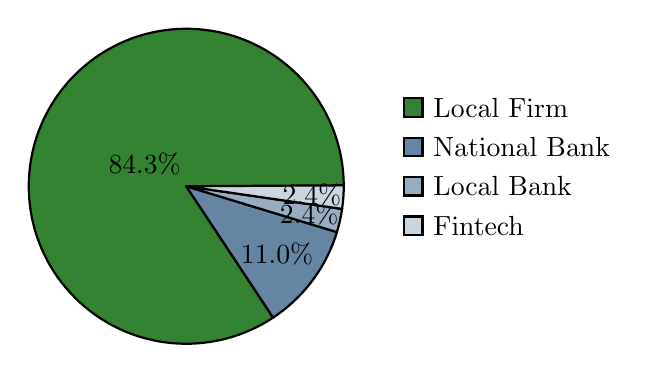
\begin{tikzpicture}
            \pie[radius=2, color={SafeGreen!80, DeepBlue!60, DeepBlue!40, DeepBlue!20}, text=legend]{
                84.3/Local Firm,
                11.0/National Bank,
                2.4/Local Bank,
                2.4/Fintech
            }
        \end{tikzpicture}
        
        \vspace{0.3cm}
        \small{\textit{Blocked party captures majority of gains}}
    \end{columns}
\end{frame}




\begin{frame}{Comparison of All Scenarios}
    \begin{table}
        \centering
        \tiny
        \begin{tabular}{lcccc}
            \toprule
            \textbf{Metric} & \textbf{Monopoly} & \textbf{Competition} & \textbf{Dual Network} & \textbf{Ideal} \\
             & (3F-WITH) & (4F-WITH) & (3F-Dual) & (3F-WITHOUT) \\
            \midrule
            \textbf{Welfare} & 0.706 & 1.034 & \textbf{1.433} & 1.433 \\
            Welfare Gap & -50.8\% & -27.9\% & \textcolor{SafeGreen}{\textbf{0.0\%}} & 0.0\% \\
            \midrule
            Bilateral Volume & 0.822 & 1.351 & 2.054 & 2.372 \\
            Direct Link ($W_{13}$) & 0.000 & 0.000 & \textbf{1.035} & 1.035 \\
            Alternative Adoption & --- & --- & 72.4\% & --- \\
            \midrule
            National Bank Utility & 0.202 & 0.391 & \textbf{0.988} & 0.802 \\
            Local Bank Utility & 0.441 & 0.239 & 0.256 & 0.216 \\
            Local Firm Utility & 0.202 & 0.391 & \textbf{0.988} & 0.802 \\
            Fintech Utility & +0.026 & +0.026 & \textbf{-0.003} & +0.037 \\
            \bottomrule
        \end{tabular}
    \end{table}
    
    \vspace{0.3cm}
    \begin{block}{Policy Ranking}
        \textbf{1st Best:} Remove constraint (may violate policy objectives) \\
        \textbf{2nd Best:} Alternative network (100\% recovery, preserves regulation) \\
        \textbf{3rd Best:} Competition (59.4\% recovery, 40.6\% gap remains)
    \end{block}
\end{frame}

% ===================================================================
% SECCIÓN 8: POLICY IMPLICATIONS
% ===================================================================
\section{Policy Implications}

\begin{frame}{Main Conclusions}
    \begin{enumerate}
        \item \textbf{Competition Alone Is Insufficient}
        \begin{itemize}
            \item Competition reduces rents but cannot eliminate structural inefficiency
            \item Persistent 40.6\% welfare gap when constraint binds
        \end{itemize}
        
        \vspace{0.3cm}
        \item \textbf{Coexistence, Not Total Migration}
        \begin{itemize}
            \item Optimal outcome: 47.9\% Alternative, 52.1\% Traditional
            \item Both networks serve complementary roles
        \end{itemize}
        
        \vspace{0.3cm}
        \item \textbf{Competition and Infrastructure Are Complementary}
        \begin{itemize}
            \item Competition reduces Alternative adoption (72.4\% → 47.9\%)
            \item But welfare recovery remains complete (100\%)
        \end{itemize}
    \end{enumerate}
\end{frame}

% ===================================================================
% SECCIÓN 9: CONCLUSIÓN
% ===================================================================
\section{Conclusion}

\begin{frame}{Contributions}
    \textbf{Theoretical Contribution:}
    \begin{itemize}
        \item Model of \textbf{dual-network equilibria} under asymmetric regulation
        \item Extension of Jalan et al. (2024) to dual-infrastructure settings
    \end{itemize}
    
    \vspace{0.5cm}
    \textbf{Main Findings:}
    \begin{enumerate}
        \item Alternative infrastructure achieves \textbf{complete welfare recovery} (100\%)
        \item Competition alone is insufficient (40.6\% gap remains)
        \item Optimal outcome: \textbf{coexistence} (52.1\% Traditional, 47.9\% Alternative)
        \item Blocked party captures 84.3\% of gains in our example
    \end{enumerate}
    
\end{frame}

\begin{frame}
    \centering
    \Huge \textbf{Thank You}
    
    \vspace{1cm}
    
    \vspace{0.5cm}
    \normalsize
    Sebastián Cea \& Hernán Venegas \\
    Universidad de Los Andes
    
\end{frame}

\begin{frame}[allowframebreaks]{References}
\begin{thebibliography}{9}
\bibitem{jalan2024}
Jalan, A., Chakrabarti, D., \& Sarkar, P. (2024). 
\textit{Incentive-Aware Models of Financial Networks}. 
Operations Research, Articles in Advance.



\bibitem{market_research_future2024}
Market Research Future. (2024). 
\textit{Global Blockchain FinTech Market Research Report}.

\end{thebibliography}
\end{frame}

\end{document}